\section{Naive Construction}

The simplest way to construct a suffix tree is to first construct a suffix trie and convert it to a suffix tree by repeatedly coalescing the paths. This takes $O(n^2)$ time and space. It takes $O(n^2)$ space because we need to store the intermediate suffix trie.

\section{Ukkonen's Linear-Time Construction}

\subsection{Types of Extensions}

Suppose that we have $S[j\ldots i] = \beta$ be a suffix of $S[1\ldots i]$. In some iteration $j$, the algorithm finds the end of $\beta$ and extends the path by adding $S[i+1]$ to the path. This ensures that the suffix $S[j\ldots i+1]$ is included in the new tree. Observe that there are three types of insertions:

\begin{enumerate}
    \item[Type 1.] In the current tree, path $\beta$ \textit{\textbf{leads to a leaf}}. In this case, $S[i+1]$ is \textit{\textbf{added to the end of the label}} on that edge.
    \begin{marginfigure}
        \centering
        \includegraphics[width=0.7\linewidth]{suffix-tree/ukkonen-type-1-insertion.pdf}
        \caption{Type 1 insertion for suffix $bx$ of $S=axabx$.}
        \hfill \\
    \end{marginfigure}

    \item[Type 2.] There is \textit{\textbf{no path}} from the end of $\beta$ that starts with character $S[i+1]$, but at least one labeled path continues from the end of $\beta$. In this case, a \textit{\textbf{new leaf edge}} starting from the end of $\beta$ is created and labeled $S[i+1]$, which leads to a \textit{\textbf{new leaf node}} with number $j$.
    \begin{marginfigure}
        \centering
        \includegraphics[width=0.7\linewidth]{suffix-tree/ukkonen-type-2-insertion.pdf}
        \caption{Type 2 insertion for suffix $x$ of $S=axabx$.}
    \end{marginfigure}

    \item[Type 3.] Some \textit{\textbf{path}} from the end of $\beta$ starts with character $S[i+1]$. In this case, $\beta \cdot S[i+1]$ is \textit{\textbf{already in the implicit suffix tree}}. So we \textit{\textbf{do nothing}}.
\end{enumerate}

\subsection{Suffix Links}

\begin{definition}[Suffix Link] \index{suffix link}
    \normalfont
    Let $x\alpha$ be an arbitrary string, where $x \in \Sigma$ is a \textit{single character} and $\alpha \in \Sigma^*$ is a (possibly empty) \textit{substring}. For an internal node $v$ with root-to-node path label $x \alpha$, if there is another node $s(v)$ with root-to-node path label $\alpha$, then we create a pointer from $v$ to $s(v)$, called a \textit{\textbf{suffix link}}.
    \begin{marginfigure}
        \centering
        \includegraphics[width=0.6\linewidth]{suffix-tree/ukkonen-suffix-link.pdf}
        \caption{A suffix link from $v$ (representing $xab$) to $s(v)$ (representing $ab$). The other two suffix links are also shown. Note that if a node's path label has no proper suffix, we create a link to the root.}
    \end{marginfigure}
\end{definition}

The reason we have suffix link is because we want to \textit{access the insertion point (end of a suffix) efficiently}. Suppose we insert a new character to the sequence $x\alpha$. Once we inserted the new character to the suffix $x \alpha$, we also need to insert the character to the end of $\alpha$. Without suffix link, we would have to traverse back to the root and search for the insertion point all over again. The use of suffix link is especially useful for jumping from one suffix to the next during extension.

\begin{figure}
    \centering
    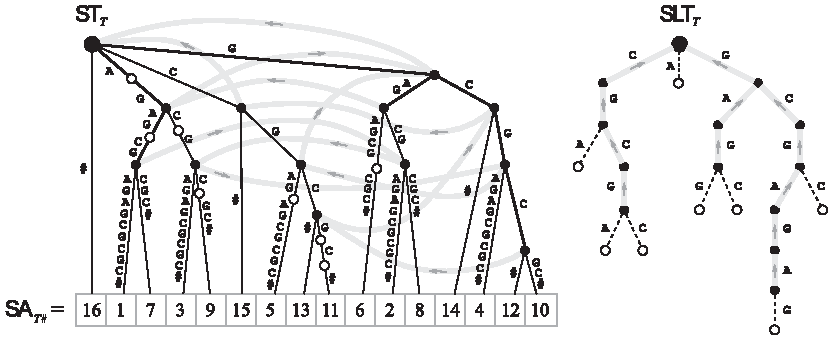
\includegraphics[width=\linewidth]{suffix-tree/st-slt-example.pdf}
    \caption{A suffix tree and its corresponding suffix link tree for $T = \texttt{AGAGCGAGAGCGCGC}$. }
\end{figure}

Moreover, the suffix links induce a subtree called the \textit{\textbf{suffix link tree}}. More formally, given a text $T$ represented by a suffix tree $(V,E)$ with suffix links, let $\ell(v)$ denote the label on the path from the root to $v$. Then, $L = \{(v,a) \mid v \in V, s(v) \in V, \ell(v) = x \ell(s(v)), x \in \Sigma\}$ be the set of all suffix links, and we define the tree $\text{SLT}(T) = (V,L)$ labeled by $\ell$ as the \textit{\textbf{suffix link tree}}.

\subsection{Count and Skip}

After reaching $s(v)$ via a suffix link, we still need to travel down the path labeled $\gamma$ in order to add a new character at the end of $\gamma$, either by branching off or creating a new leaf node. However, this walk along the $\gamma$ path takes $O(|\gamma|)$ if implemented directly. An alternative to this would be to \textit{\textbf{store the number of characters of on each edge}} and skip nodes wheneve we can.

Let $g$ denote the length of $\gamma$, the next suffix to which we want to append the new character. We start the search for the insertion point starting from $s(v)$.

\begin{marginfigure}
    \centering
    \includegraphics[width=0.8\linewidth]{suffix-tree/ukkonen-count-skip.pdf}
    \caption{\\Top: Case 1 where $g \geq g'$, skip to the next node; \\ Bottom: Case 2 where $g < g'$, go the the $g$-th character on the current edge.}
\end{marginfigure}

Recall that no two edges coming out of $s(v)$ can have labels starting with the same character. We can then use one comparison to determine the edge that we need to follow. In particular, let $h=1$ initially and before each iteration, compare the $h$th character of $\gamma$ with the first character of every edge coming out of the current node. Let $g'$ be the number of characters on the edge that we have just identified. Then, consider the following two cases:

\begin{enumerate}
    \item $g \geq g'$: Skip to the node at the end of the edge. Set $g = g - g'$, $h = h + g'$, and repeat.
    \item $g < g'$: Skip to the $g$th character on the edge and stop.
\end{enumerate}

\subsection{Edge Label Compression}

Another issue with our high-level ``algorithm'' for Ukkonen's algorithm is that every edge is explicitly labeled with the suffix they represent. A label of an edge can be as large as $\Theta(m)$, and there can be at most $\Theta(m)$ edges, making the total space required for a suffix tree $\Theta(m^2)$ in this case. This makes it impossible to build such a tree in $O(m)$ time. Fortunately, this issue can be solved using a simple trick: instead of storing the strings explicitly, we can store a pair of indicies representing the \textit{\textbf{starting and ending position of the substring}} represented by each edge. That way, each edge can be maintained using only $\Theta(\log m)$ space.

\index{word RAM model}
In the \textit{\textbf{word RAM model}}\footnote{In complexity theory, we have focused on Turing machine as our preferred model of computation. However, in analysis of algorithms, we usually use the word RAM model (often without explicitly stating it) as it is a more realistic model of how modern computers work.}, we assume that every word of size $\log m$ bits can be read and written efficiently in constant time. Hence, it is more plausible to build a suffix tree with compressed edge labels in linear time.

\subsection{Key Observations}

\newthought{No More Insertions After Type 3}

In any given phase $i+1$, if there is a Type 3 extension $j$ (the new suffix $S[j\ldots i+1]$ is already in the tree), then any further extensions in the current phase will also be of Type 3. When there is a Type 3 extension, the path labeled $S[j\ldots i]$ in the current tree must have already contained $S[i+1]$. Then clearly, so does $S[j'\ldots i]$ for all $j < j' \leq i+1$ because they are all suffixes of $S[j\ldots i]$.

\newthought{Once a Leaf, Always a Leaf}

At some point in the algorithm, if a leaf $j$ is created for the suffix starting at position $j$, then the leaf will remain a leaf throughout the algorithm. This is because the algorithm never extends a leaf. If a path leads to a leaf, it will be a Type 1 insertion, in which case we extend the edge label without explicitly adding new nodes.